\XtoCBlock{TDSystemO2}
\label{block:TDSystemO2}
\begin{figure}[H]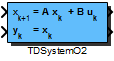
\includegraphics{TDSystemO2}\end{figure} 

\begin{XtoCtabular}{Inports}
In1 & Input \#1\tabularnewline
\hline
In2 & Input \#2\tabularnewline
\hline
\end{XtoCtabular}


\begin{XtoCtabular}{Outports}
Out1 & Output \#1\tabularnewline
\hline
Out2 & Output \#2\tabularnewline
\hline
\end{XtoCtabular}

\begin{XtoCtabular}{Mask Parameters}
A & State matrix A\tabularnewline
\hline
B & Input matrix B\tabularnewline
\hline
\end{XtoCtabular}

\subsubsection*{Description:}
2nd order time discrete system with two inputs and two outputs.

% include optional documentation file
\InputIfFileExists{\XcHomePath/Library/Control/Doc/TDSystemO2_Info.tex}{\vspace{1ex}}{}

\subsubsection*{Implementations:}
\begin{tabular}{l l}
\textbf{FiP8} & 8 Bit Fixed Point Implementation\tabularnewline
\textbf{FiP16} & 16 Bit Fixed Point Implementation\tabularnewline
\textbf{FiP32} & 32 Bit Fixed Point Implementation\tabularnewline
\textbf{Float32} & 32 Bit Floating Point Implementation\tabularnewline
\textbf{Float64} & 64 Bit Floating Point Implementation\tabularnewline
\end{tabular}

\XtoCImplementation{FiP8}
\index{Block ID!3360}
\nopagebreak[0]
% Implementation details
\begin{tabular}{l l}
\textbf{Name} & FiP8 \tabularnewline
\textbf{ID} & 3360 \tabularnewline
\textbf{Revision} & 1 \tabularnewline
\textbf{C filename} & TDSystemO2\_FiP8.c \tabularnewline
\textbf{H filename} & TDSystemO2\_FiP8.h \tabularnewline
\end{tabular}
\vspace{1ex}

8 Bit Fixed Point Implementation

\begin{XtoCtabular}{Controller Parameters}
a11 & Coefficient a11\tabularnewline
\hline
a12 & Coefficient a12\tabularnewline
\hline
a21 & Coefficient a21\tabularnewline
\hline
a22 & Coefficient a22\tabularnewline
\hline
b11 & Coefficient b11\tabularnewline
\hline
b12 & Coefficient b12\tabularnewline
\hline
b21 & Coefficient b21\tabularnewline
\hline
b22 & Coefficient b22\tabularnewline
\hline
sfra11 & Shift factor for coefficient a11\tabularnewline
\hline
sfra12 & Shift factor for coefficient a12\tabularnewline
\hline
sfra21 & Shift factor for coefficient a21\tabularnewline
\hline
sfra22 & Shift factor for coefficient a22\tabularnewline
\hline
sfrb11 & Shift factor for coefficient b11\tabularnewline
\hline
sfrb12 & Shift factor for coefficient b12\tabularnewline
\hline
sfrb21 & Shift factor for coefficient b21\tabularnewline
\hline
sfrb22 & Shift factor for coefficient b22\tabularnewline
\hline
x1 & State x1\tabularnewline
\hline
x2 & State x2\tabularnewline
\hline
\end{XtoCtabular}

% Implementation data structure
\XtoCDataStruct{Data Structure:}
\begin{lstlisting}
typedef struct {
     uint16        ID;
     int8          *In1;
     int8          *In2;
     int8          Out1;
     int8          Out2;
     int8          a11;
     int8          a12;
     int8          a21;
     int8          a22;
     int8          b11;
     int8          b12;
     int8          b21;
     int8          b22;
     uint8         sfra11;
     uint8         sfra12;
     uint8         sfra21;
     uint8         sfra22;
     uint8         sfrb11;
     uint8         sfrb12;
     uint8         sfrb21;
     uint8         sfrb22;
     int8          x1;
     int8          x2;
} TDSYSTEMO2_FIP8;
\end{lstlisting}

\ifdefined \AddTestReports
\InputIfFileExists{\XcHomePath/Library/Control/Doc/Test_TDSystemO2_FiP8.tex}{}{}
\fi
\XtoCImplementation{FiP16}
\index{Block ID!3361}
\nopagebreak[0]
% Implementation details
\begin{tabular}{l l}
\textbf{Name} & FiP16 \tabularnewline
\textbf{ID} & 3361 \tabularnewline
\textbf{Revision} & 1 \tabularnewline
\textbf{C filename} & TDSystemO2\_FiP16.c \tabularnewline
\textbf{H filename} & TDSystemO2\_FiP16.h \tabularnewline
\end{tabular}
\vspace{1ex}

16 Bit Fixed Point Implementation

\begin{XtoCtabular}{Controller Parameters}
a11 & Coefficient a11\tabularnewline
\hline
a12 & Coefficient a12\tabularnewline
\hline
a21 & Coefficient a21\tabularnewline
\hline
a22 & Coefficient a22\tabularnewline
\hline
b11 & Coefficient b11\tabularnewline
\hline
b12 & Coefficient b12\tabularnewline
\hline
b21 & Coefficient b21\tabularnewline
\hline
b22 & Coefficient b22\tabularnewline
\hline
sfra11 & Shift factor for coefficient a11\tabularnewline
\hline
sfra12 & Shift factor for coefficient a12\tabularnewline
\hline
sfra21 & Shift factor for coefficient a21\tabularnewline
\hline
sfra22 & Shift factor for coefficient a22\tabularnewline
\hline
sfrb11 & Shift factor for coefficient b11\tabularnewline
\hline
sfrb12 & Shift factor for coefficient b12\tabularnewline
\hline
sfrb21 & Shift factor for coefficient b21\tabularnewline
\hline
sfrb22 & Shift factor for coefficient b22\tabularnewline
\hline
x1 & State x1\tabularnewline
\hline
x2 & State x2\tabularnewline
\hline
\end{XtoCtabular}

% Implementation data structure
\XtoCDataStruct{Data Structure:}
\begin{lstlisting}
typedef struct {
     uint16        ID;
     int16         *In1;
     int16         *In2;
     int16         Out1;
     int16         Out2;
     int16         a11;
     int16         a12;
     int16         a21;
     int16         a22;
     int16         b11;
     int16         b12;
     int16         b21;
     int16         b22;
     uint8         sfra11;
     uint8         sfra12;
     uint8         sfra21;
     uint8         sfra22;
     uint8         sfrb11;
     uint8         sfrb12;
     uint8         sfrb21;
     uint8         sfrb22;
     int16         x1;
     int16         x2;
} TDSYSTEMO2_FIP16;
\end{lstlisting}

\ifdefined \AddTestReports
\InputIfFileExists{\XcHomePath/Library/Control/Doc/Test_TDSystemO2_FiP16.tex}{}{}
\fi
\XtoCImplementation{FiP32}
\index{Block ID!3362}
\nopagebreak[0]
% Implementation details
\begin{tabular}{l l}
\textbf{Name} & FiP32 \tabularnewline
\textbf{ID} & 3362 \tabularnewline
\textbf{Revision} & 1 \tabularnewline
\textbf{C filename} & TDSystemO2\_FiP32.c \tabularnewline
\textbf{H filename} & TDSystemO2\_FiP32.h \tabularnewline
\end{tabular}
\vspace{1ex}

32 Bit Fixed Point Implementation

\begin{XtoCtabular}{Controller Parameters}
a11 & Coefficient a11\tabularnewline
\hline
a12 & Coefficient a12\tabularnewline
\hline
a21 & Coefficient a21\tabularnewline
\hline
a22 & Coefficient a22\tabularnewline
\hline
b11 & Coefficient b11\tabularnewline
\hline
b12 & Coefficient b12\tabularnewline
\hline
b21 & Coefficient b21\tabularnewline
\hline
b22 & Coefficient b22\tabularnewline
\hline
sfra11 & Shift factor for coefficient a11\tabularnewline
\hline
sfra12 & Shift factor for coefficient a12\tabularnewline
\hline
sfra21 & Shift factor for coefficient a21\tabularnewline
\hline
sfra22 & Shift factor for coefficient a22\tabularnewline
\hline
sfrb11 & Shift factor for coefficient b11\tabularnewline
\hline
sfrb12 & Shift factor for coefficient b12\tabularnewline
\hline
sfrb21 & Shift factor for coefficient b21\tabularnewline
\hline
sfrb22 & Shift factor for coefficient b22\tabularnewline
\hline
x1 & State x1\tabularnewline
\hline
x2 & State x2\tabularnewline
\hline
\end{XtoCtabular}

% Implementation data structure
\XtoCDataStruct{Data Structure:}
\begin{lstlisting}
typedef struct {
     uint16        ID;
     int32         *In1;
     int32         *In2;
     int32         Out1;
     int32         Out2;
     int32         a11;
     int32         a12;
     int32         a21;
     int32         a22;
     int32         b11;
     int32         b12;
     int32         b21;
     int32         b22;
     uint8         sfra11;
     uint8         sfra12;
     uint8         sfra21;
     uint8         sfra22;
     uint8         sfrb11;
     uint8         sfrb12;
     uint8         sfrb21;
     uint8         sfrb22;
     int32         x1;
     int32         x2;
} TDSYSTEMO2_FIP32;
\end{lstlisting}

\ifdefined \AddTestReports
\InputIfFileExists{\XcHomePath/Library/Control/Doc/Test_TDSystemO2_FiP32.tex}{}{}
\fi
\XtoCImplementation{Float32}
\index{Block ID!3363}
\nopagebreak[0]
% Implementation details
\begin{tabular}{l l}
\textbf{Name} & Float32 \tabularnewline
\textbf{ID} & 3363 \tabularnewline
\textbf{Revision} & 0.1 \tabularnewline
\textbf{C filename} & TDSystemO2\_Float32.c \tabularnewline
\textbf{H filename} & TDSystemO2\_Float32.h \tabularnewline
\end{tabular}
\vspace{1ex}

32 Bit Floating Point Implementation

\begin{XtoCtabular}{Controller Parameters}
a11 & Coefficient a11\tabularnewline
\hline
a12 & Coefficient a12\tabularnewline
\hline
a21 & Coefficient a21\tabularnewline
\hline
a22 & Coefficient a22\tabularnewline
\hline
b11 & Coefficient b11\tabularnewline
\hline
b12 & Coefficient b12\tabularnewline
\hline
b21 & Coefficient b21\tabularnewline
\hline
b22 & Coefficient b22\tabularnewline
\hline
x1 & State x1\tabularnewline
\hline
x2 & State x2\tabularnewline
\hline
\end{XtoCtabular}

% Implementation data structure
\XtoCDataStruct{Data Structure:}
\begin{lstlisting}
typedef struct {
     uint16        ID;
     float32       *In1;
     float32       *In2;
     float32       Out1;
     float32       Out2;
     float32       a11;
     float32       a12;
     float32       a21;
     float32       a22;
     float32       b11;
     float32       b12;
     float32       b21;
     float32       b22;
     float32       x1;
     float32       x2;
} TDSYSTEMO2_FLOAT32;
\end{lstlisting}

\ifdefined \AddTestReports
\InputIfFileExists{\XcHomePath/Library/Control/Doc/Test_TDSystemO2_Float32.tex}{}{}
\fi
\XtoCImplementation{Float64}
\index{Block ID!3364}
\nopagebreak[0]
% Implementation details
\begin{tabular}{l l}
\textbf{Name} & Float64 \tabularnewline
\textbf{ID} & 3364 \tabularnewline
\textbf{Revision} & 0.1 \tabularnewline
\textbf{C filename} & TDSystemO2\_Float64.c \tabularnewline
\textbf{H filename} & TDSystemO2\_Float64.h \tabularnewline
\end{tabular}
\vspace{1ex}

64 Bit Floating Point Implementation

\begin{XtoCtabular}{Controller Parameters}
a11 & Coefficient a11\tabularnewline
\hline
a12 & Coefficient a12\tabularnewline
\hline
a21 & Coefficient a21\tabularnewline
\hline
a22 & Coefficient a22\tabularnewline
\hline
b11 & Coefficient b11\tabularnewline
\hline
b12 & Coefficient b12\tabularnewline
\hline
b21 & Coefficient b21\tabularnewline
\hline
b22 & Coefficient b22\tabularnewline
\hline
x1 & State x1\tabularnewline
\hline
x2 & State x2\tabularnewline
\hline
\end{XtoCtabular}

% Implementation data structure
\XtoCDataStruct{Data Structure:}
\begin{lstlisting}
typedef struct {
     uint16        ID;
     float64       *In1;
     float64       *In2;
     float64       Out1;
     float64       Out2;
     float64       a11;
     float64       a12;
     float64       a21;
     float64       a22;
     float64       b11;
     float64       b12;
     float64       b21;
     float64       b22;
     float64       x1;
     float64       x2;
} TDSYSTEMO2_FLOAT64;
\end{lstlisting}

\ifdefined \AddTestReports
\InputIfFileExists{\XcHomePath/Library/Control/Doc/Test_TDSystemO2_Float64.tex}{}{}
\fi
